
Durch die Konvergenz der Magnetisierung über eine Monte Carlo Simulation kann nun das Verhalten der Magnetisierung in Abhängigkeit von äußeren Parametern wie Temperatur und Magnetfeld untersucht werden. Hier bei ist zu beachten, dass für die Kopplungskonstante und den Boltzmannfaktor im Folgenden gilt: $J=k_{b}=1$. Insbesondere folgt daraus, dass hier nur Ferromagneten betrachtet werden. Für Antiferromagneten müsste alle Simulationen mit $J=-1$ durchgeführt werden.


\subsection{Phasenübergang zwischen Hoch- und Niedertemperaturphase}

Um die Abhängigkeit der Magnetisierung von der Temperatur zu bestimmen, wird jeweils eine Monte Carlo Simulation pro Temperatur für ein konstantes Magnetfeld durch geführt.


\paragraph{2D-Modell}

\

\

Als erstes wird das 2D-Ising Modell betrachtet. Als Grundlage dient ein YYxYY Gitter. Es wird je Simulation mit einem neuen Gitter gestartet und 1000 Monte Carlo Schritte ausgeführt. 


Zunächst wird die Temperaturabhängigkeit ohne äußeres Feld ($B=0$) untersucht. Durch die analytische Lösung ist die kritische Temperatur ($T_{c}\approx 2,269$), welche den Übergang zwischen Hoch- und Niedertemperaturphase bestimmt, bekannt, sodass ohne weiteres Simulationen von $T=1,5$ bis $T=3,5$ mit einem Schritt von $\Delta T = 0.005$. Hierbei werden zunächst die unterschiedlichen Auswirkungen der Startkonfigurationen betrachtet.
\begin{figure}[H]
	\centering
	\subfigure[Start aus Zufallskonfiguration]{
		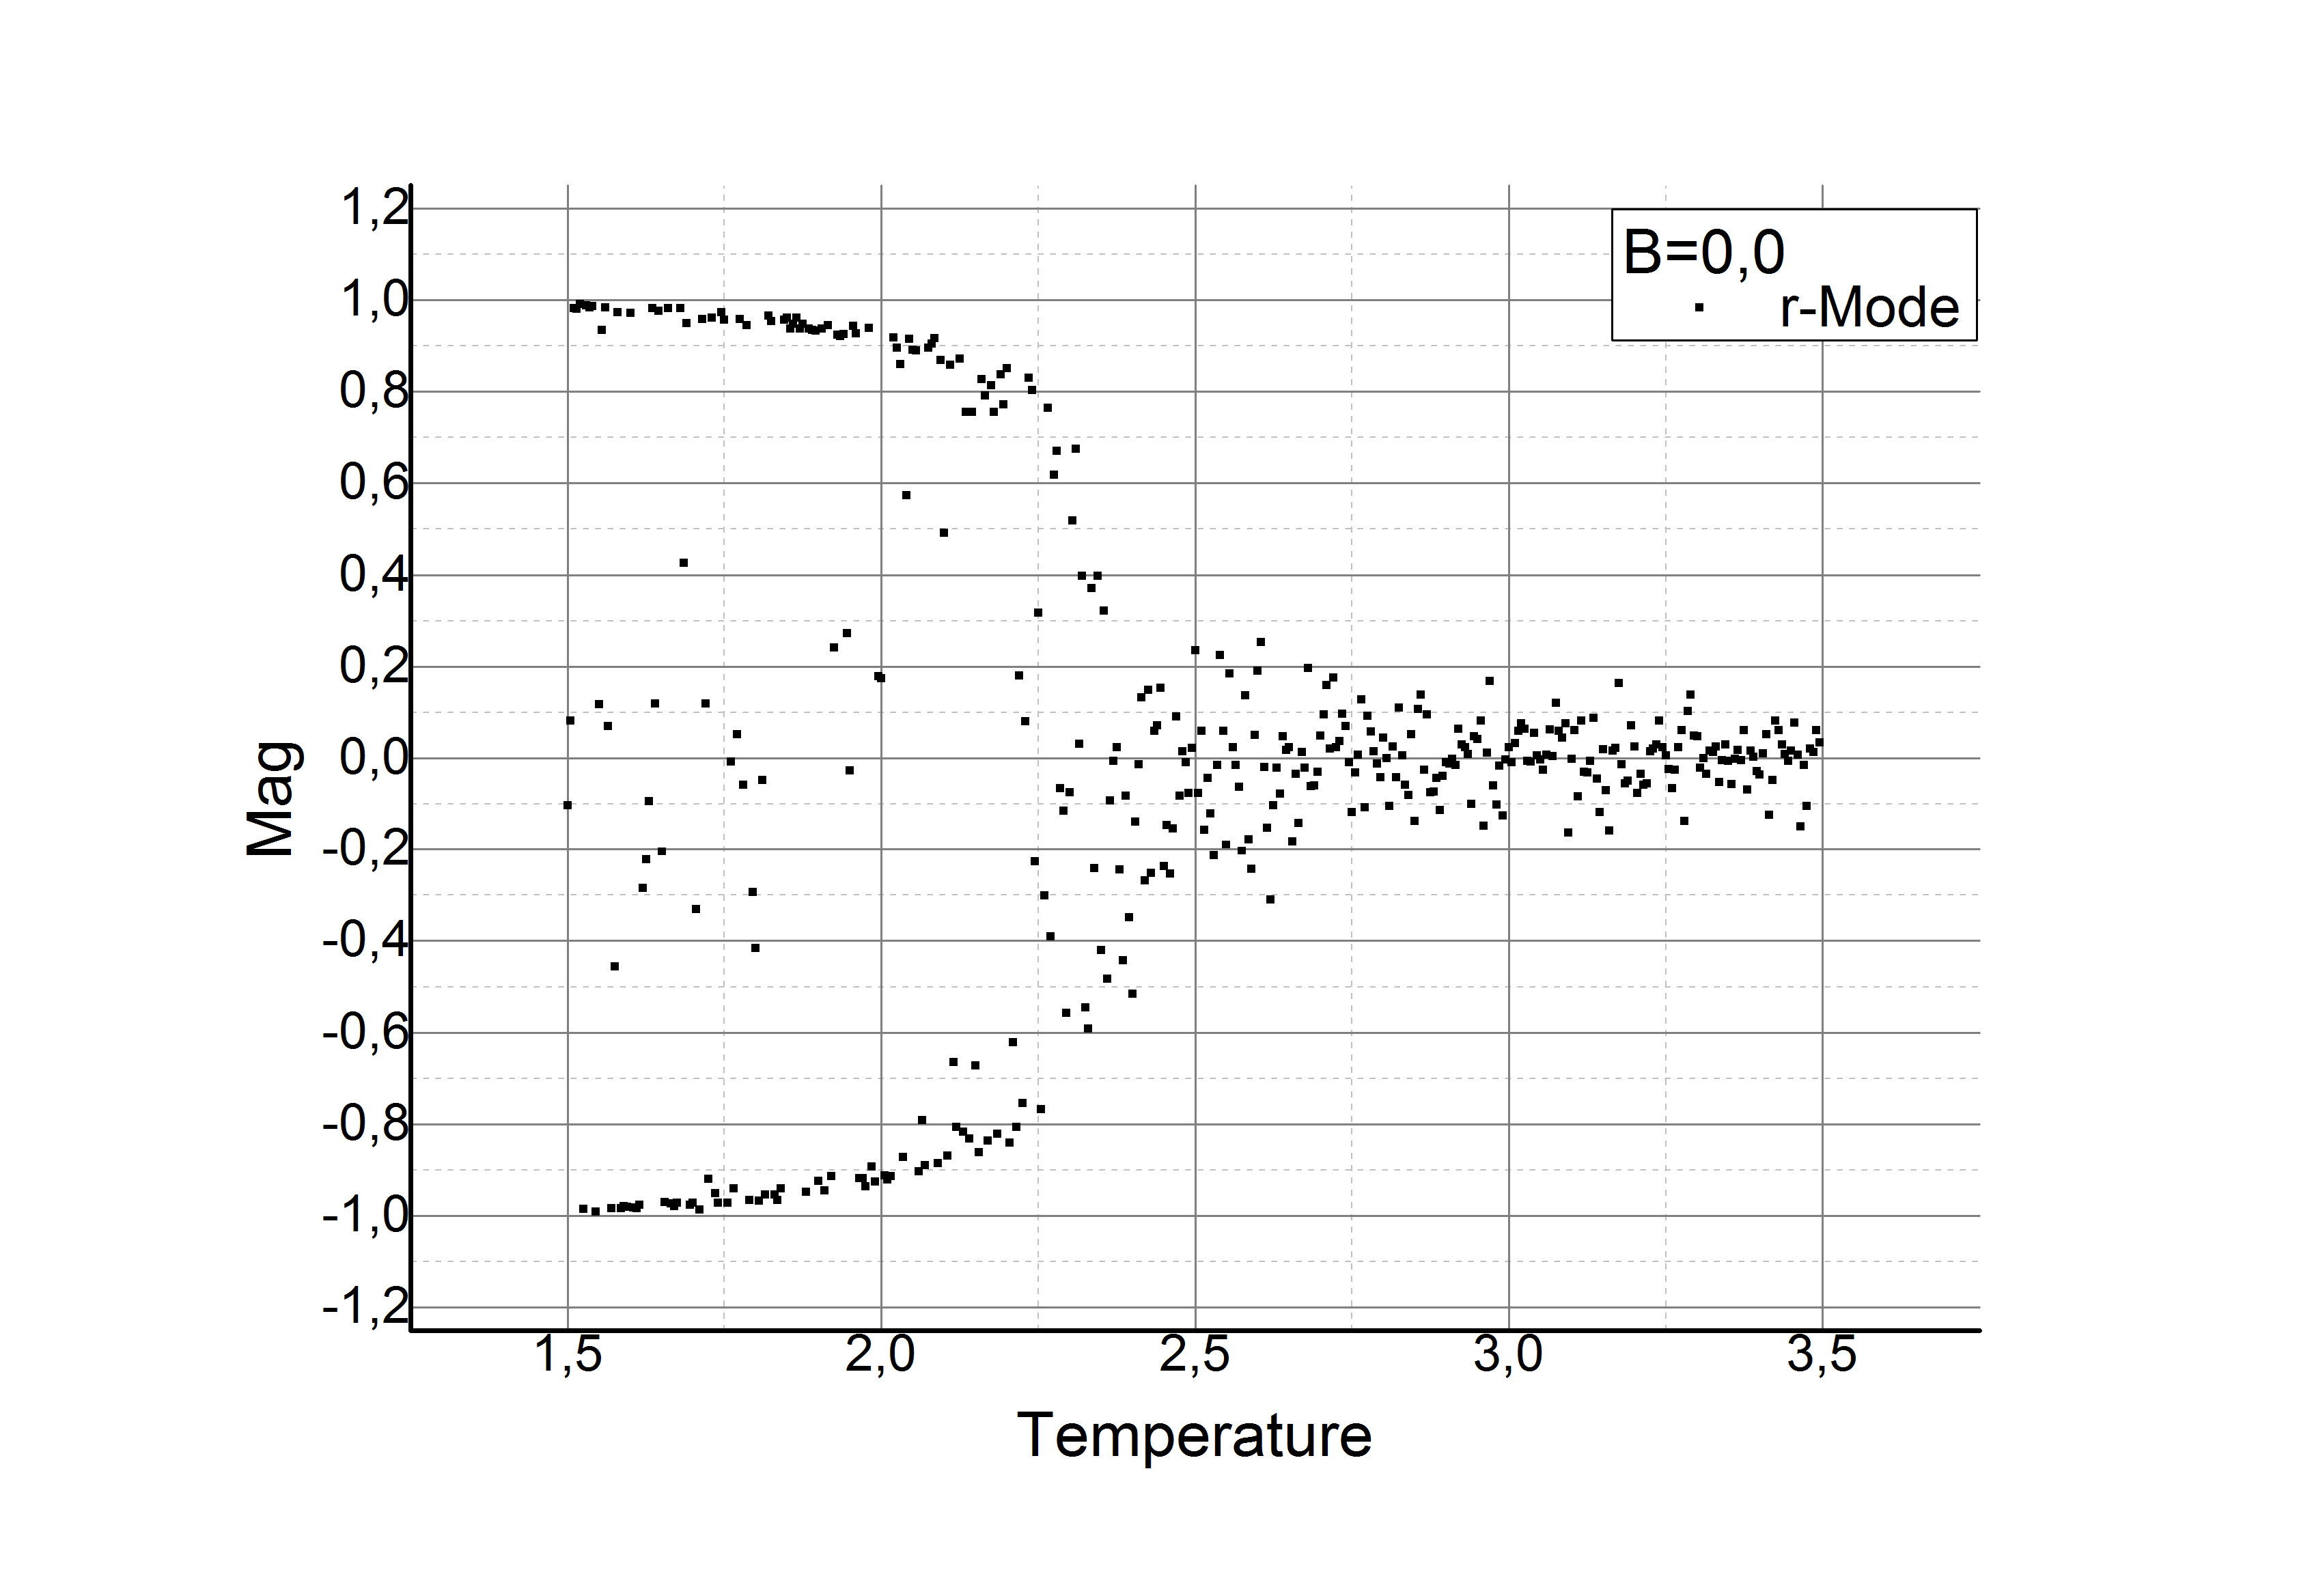
\includegraphics[width=0.47\textwidth]{../Graph_Export/MP2D/m(T)_B=0_rMode_MP2D_50_Plot.jpg}
}	
	\subfigure[Start aus geordneten Konfigurationen]{
		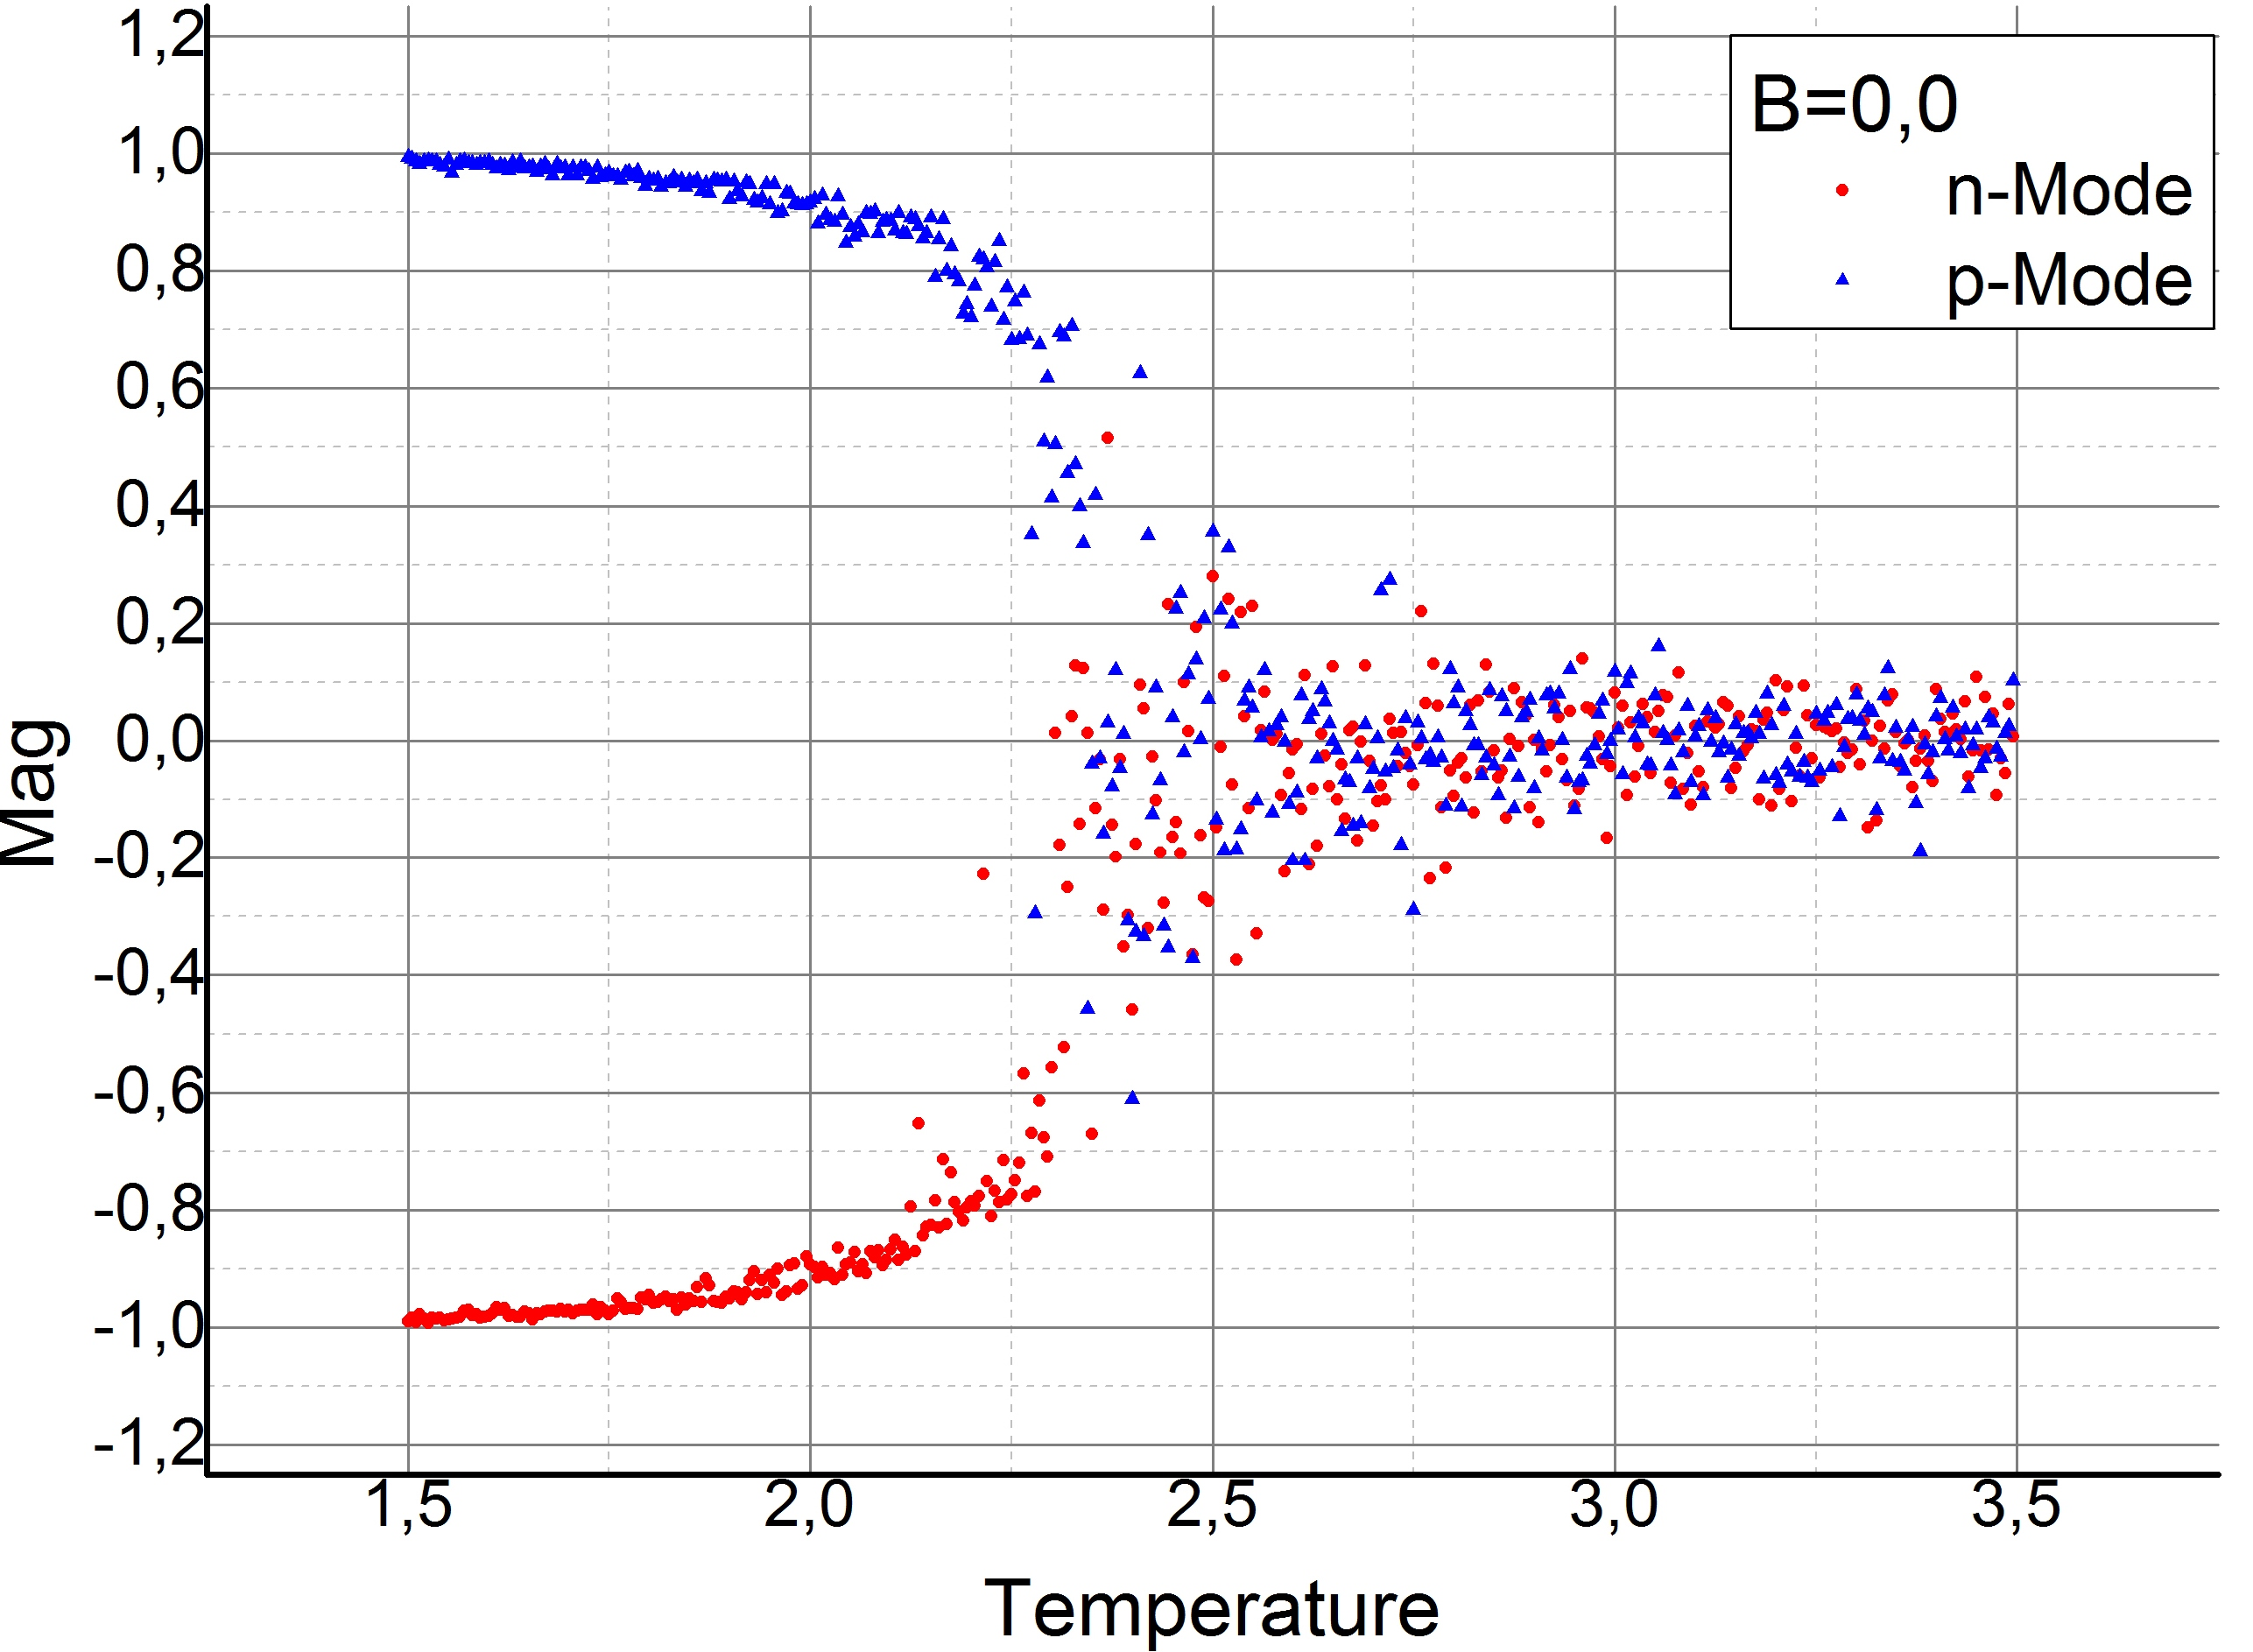
\includegraphics[width=0.47\textwidth]{../Graph_Export/MP2D/m(T)_B=0_pnModes_MP2D_50_Plot.jpg}
}		
	\caption{Temperaturabhängigkeit der Magnetisierung im 2D Ising Modells via Metropolisalgorithmus ohne äußeres Feld}
	\label{mp2d0modes}
\end{figure}
Es ist erkennbar, dass sich die Wahl der Startkonfiguration nicht auf den grundsätzlichen Verlauf der Kurve auswirkt. Dabei sollten allerdings 2 Aspekte beachtet werden. Erstens erkennt man bei Start in einer zufälligen Konfiguration einige Ausreißer im Bereich $T<T_{c}$, in denen einige Simulationen offensichtlich nicht konvergierten. Zweitens führt eine positive Startkonfiguration trivialerweise zu einer Konvergenz zum positiven Wert $m_{0}$ und umgekehrt. Gleich bleibt jedoch das große Rauschen um $T_{c}$, welches zu einer großen Ungenauigkeit bei der Bestimmung der Curie-Temperatur führt, jedoch liegt sie mit einer Abschätzung von $T_{c}\approx 2,26\pm 0,02$ absolut im erwarteten Bereich. Auch ein kleineres Rauschen für $T>T_{c}$ mit einer Bandbreite von $\pm 0,2 = 0,4$ ist in allen Simulationen vorhanden. Um dieses Rauschen zu minimieren könnte man mit größeren Gittern arbeiten, diese erzeugen jedoch auch mehr Ausreißer im Bereich $T<T_{c}$.


Für eine optimale Auflösung empfiehlt sich für Metropolis Algorithmen ohne äußeres Feld folglich zwei Simulationen, je eine aus positiver und negativer Startkonfiguration.


Nun soll die Auswirkung eines äußeren Feldes auf die Temperaturabhängigkeit betrachtet werden. Dazu wird obige Simulation für die Felder $B=\pm 0,1$ im Bereich $T=1,5$ bis $T=5,0$ und $B=\pm 0,4$ im Bereich $T=1,5$ bis $T=7,0$ durchgeführt. Dabei wird die Schrittweite auf $\Delta T = 0.01$ bzw. $\Delta T = 0.02$ erhöht. Für Simulationen mit äußerem Feld ist die Wahl der Startkonfiguration egal, da das Feld das Vorzeichen des angenommen Werts bestimmt.
\begin{figure}[H]
	\centering
	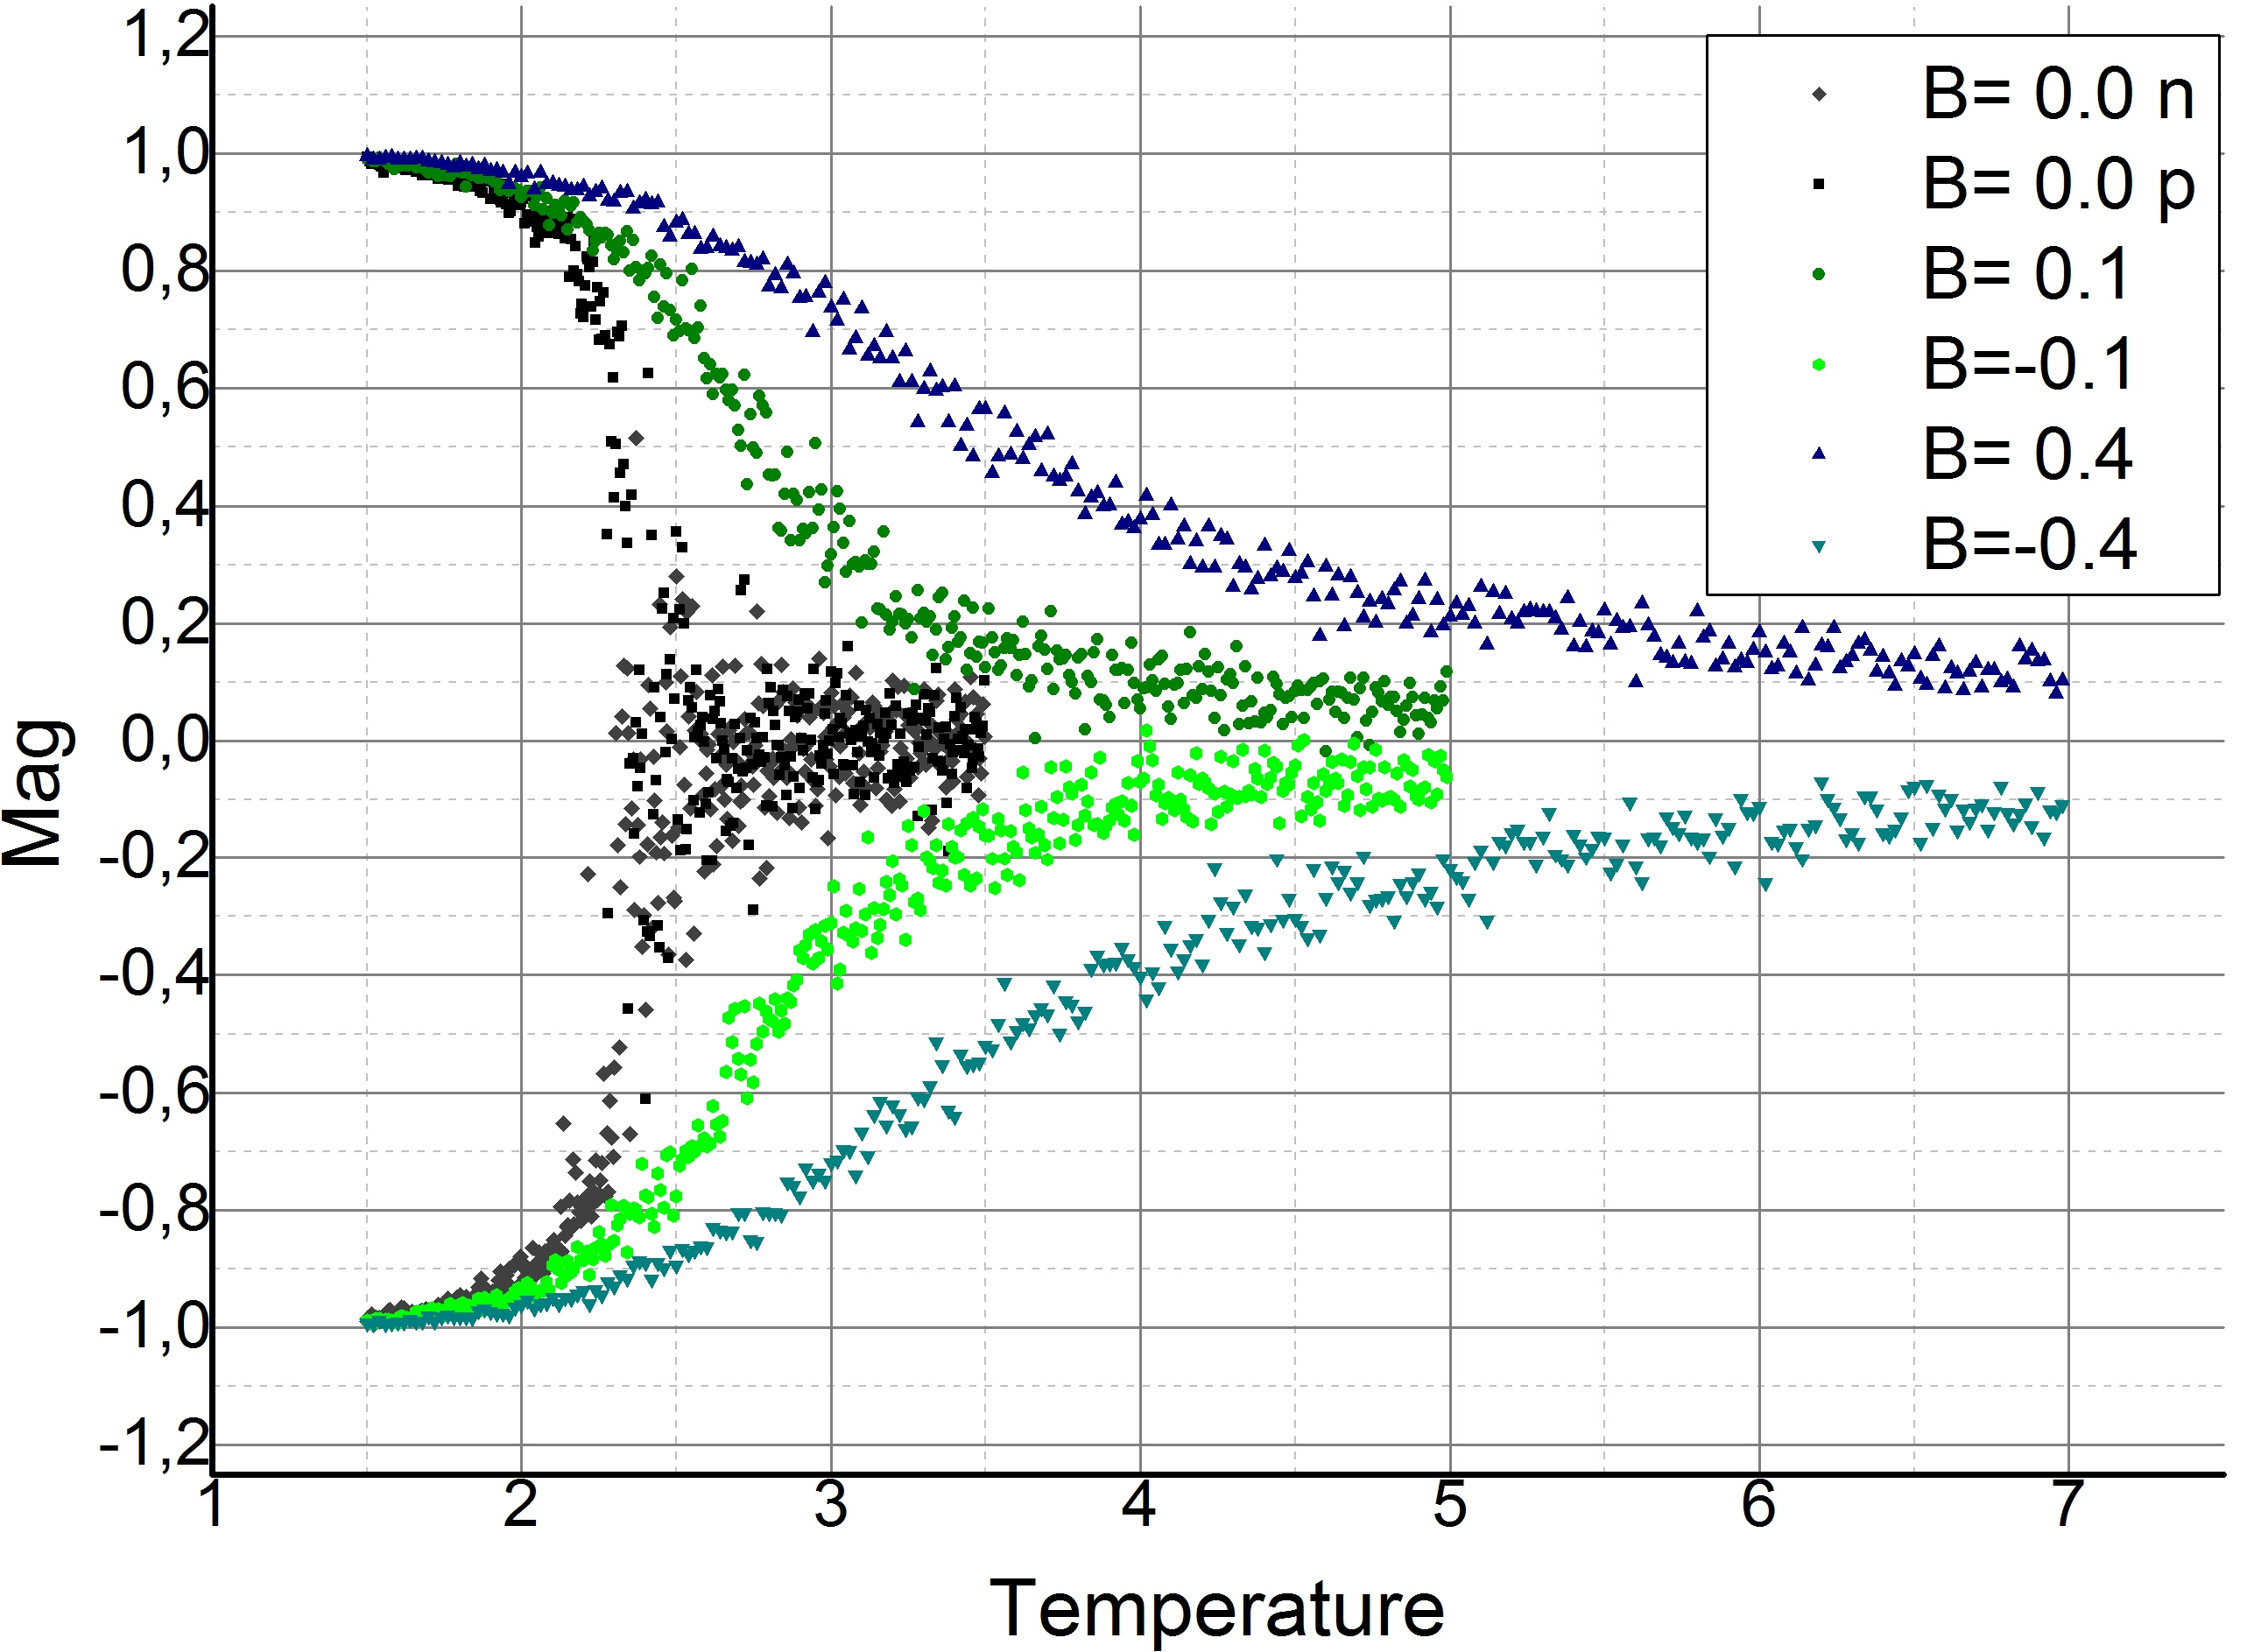
\includegraphics[width=0.8\textwidth]{../Graph_Export/MP2D/m(T)_MP2D_50_Plot.jpg}	
	\caption{Temperaturabhängigkeit der Magnetisierung im 2D Ising Modells via Metropolisalgorithmus für verschiedene äußere Felder}
	\label{mp2db}
\end{figure}
Während ohne äußeres Feld die Magnetisierung an $T_{c}$ steil abfällt und (bis auf ein Rauschen) auf Null zurückgeht, treten bei angelegtem Feld Ausschmierungen auf, sodass sich die Kurve asymptotisch der Null nähert und man weiterhin zwischen negativem und positivem Arm unterscheiden kann, welche dan jeweils mit etwa $0,2$ zum Grundrauschen beitragen. Auch nimmt die Größe der Ausschmierung bei stärkeren Feldern weiter zu.


\paragraph{3DModell}

\

\

Nun wird das die Temperatur im 3D-IsingModell untersucht. Um in vertretbarem Rechenaufwand zu bleiben, wird ein 20x20x20 Gitter benutzt. Jede Simulation startet mit einem neuem Gitter und führt wiederum 1000 Schritte aus.


Als erstes wird wieder die Auswirkung der Startkonfiguration auf Simulationen ohne äußeres Feld untersucht. Die Simulationen laufen jeweils von $T=2,5$ bis $T=6,0$ mit einer Schrittweite von $\Delta T= 0,01$.
\begin{figure}[H]
	\centering
	\subfigure[Start aus Zufallskonfiguration]{
		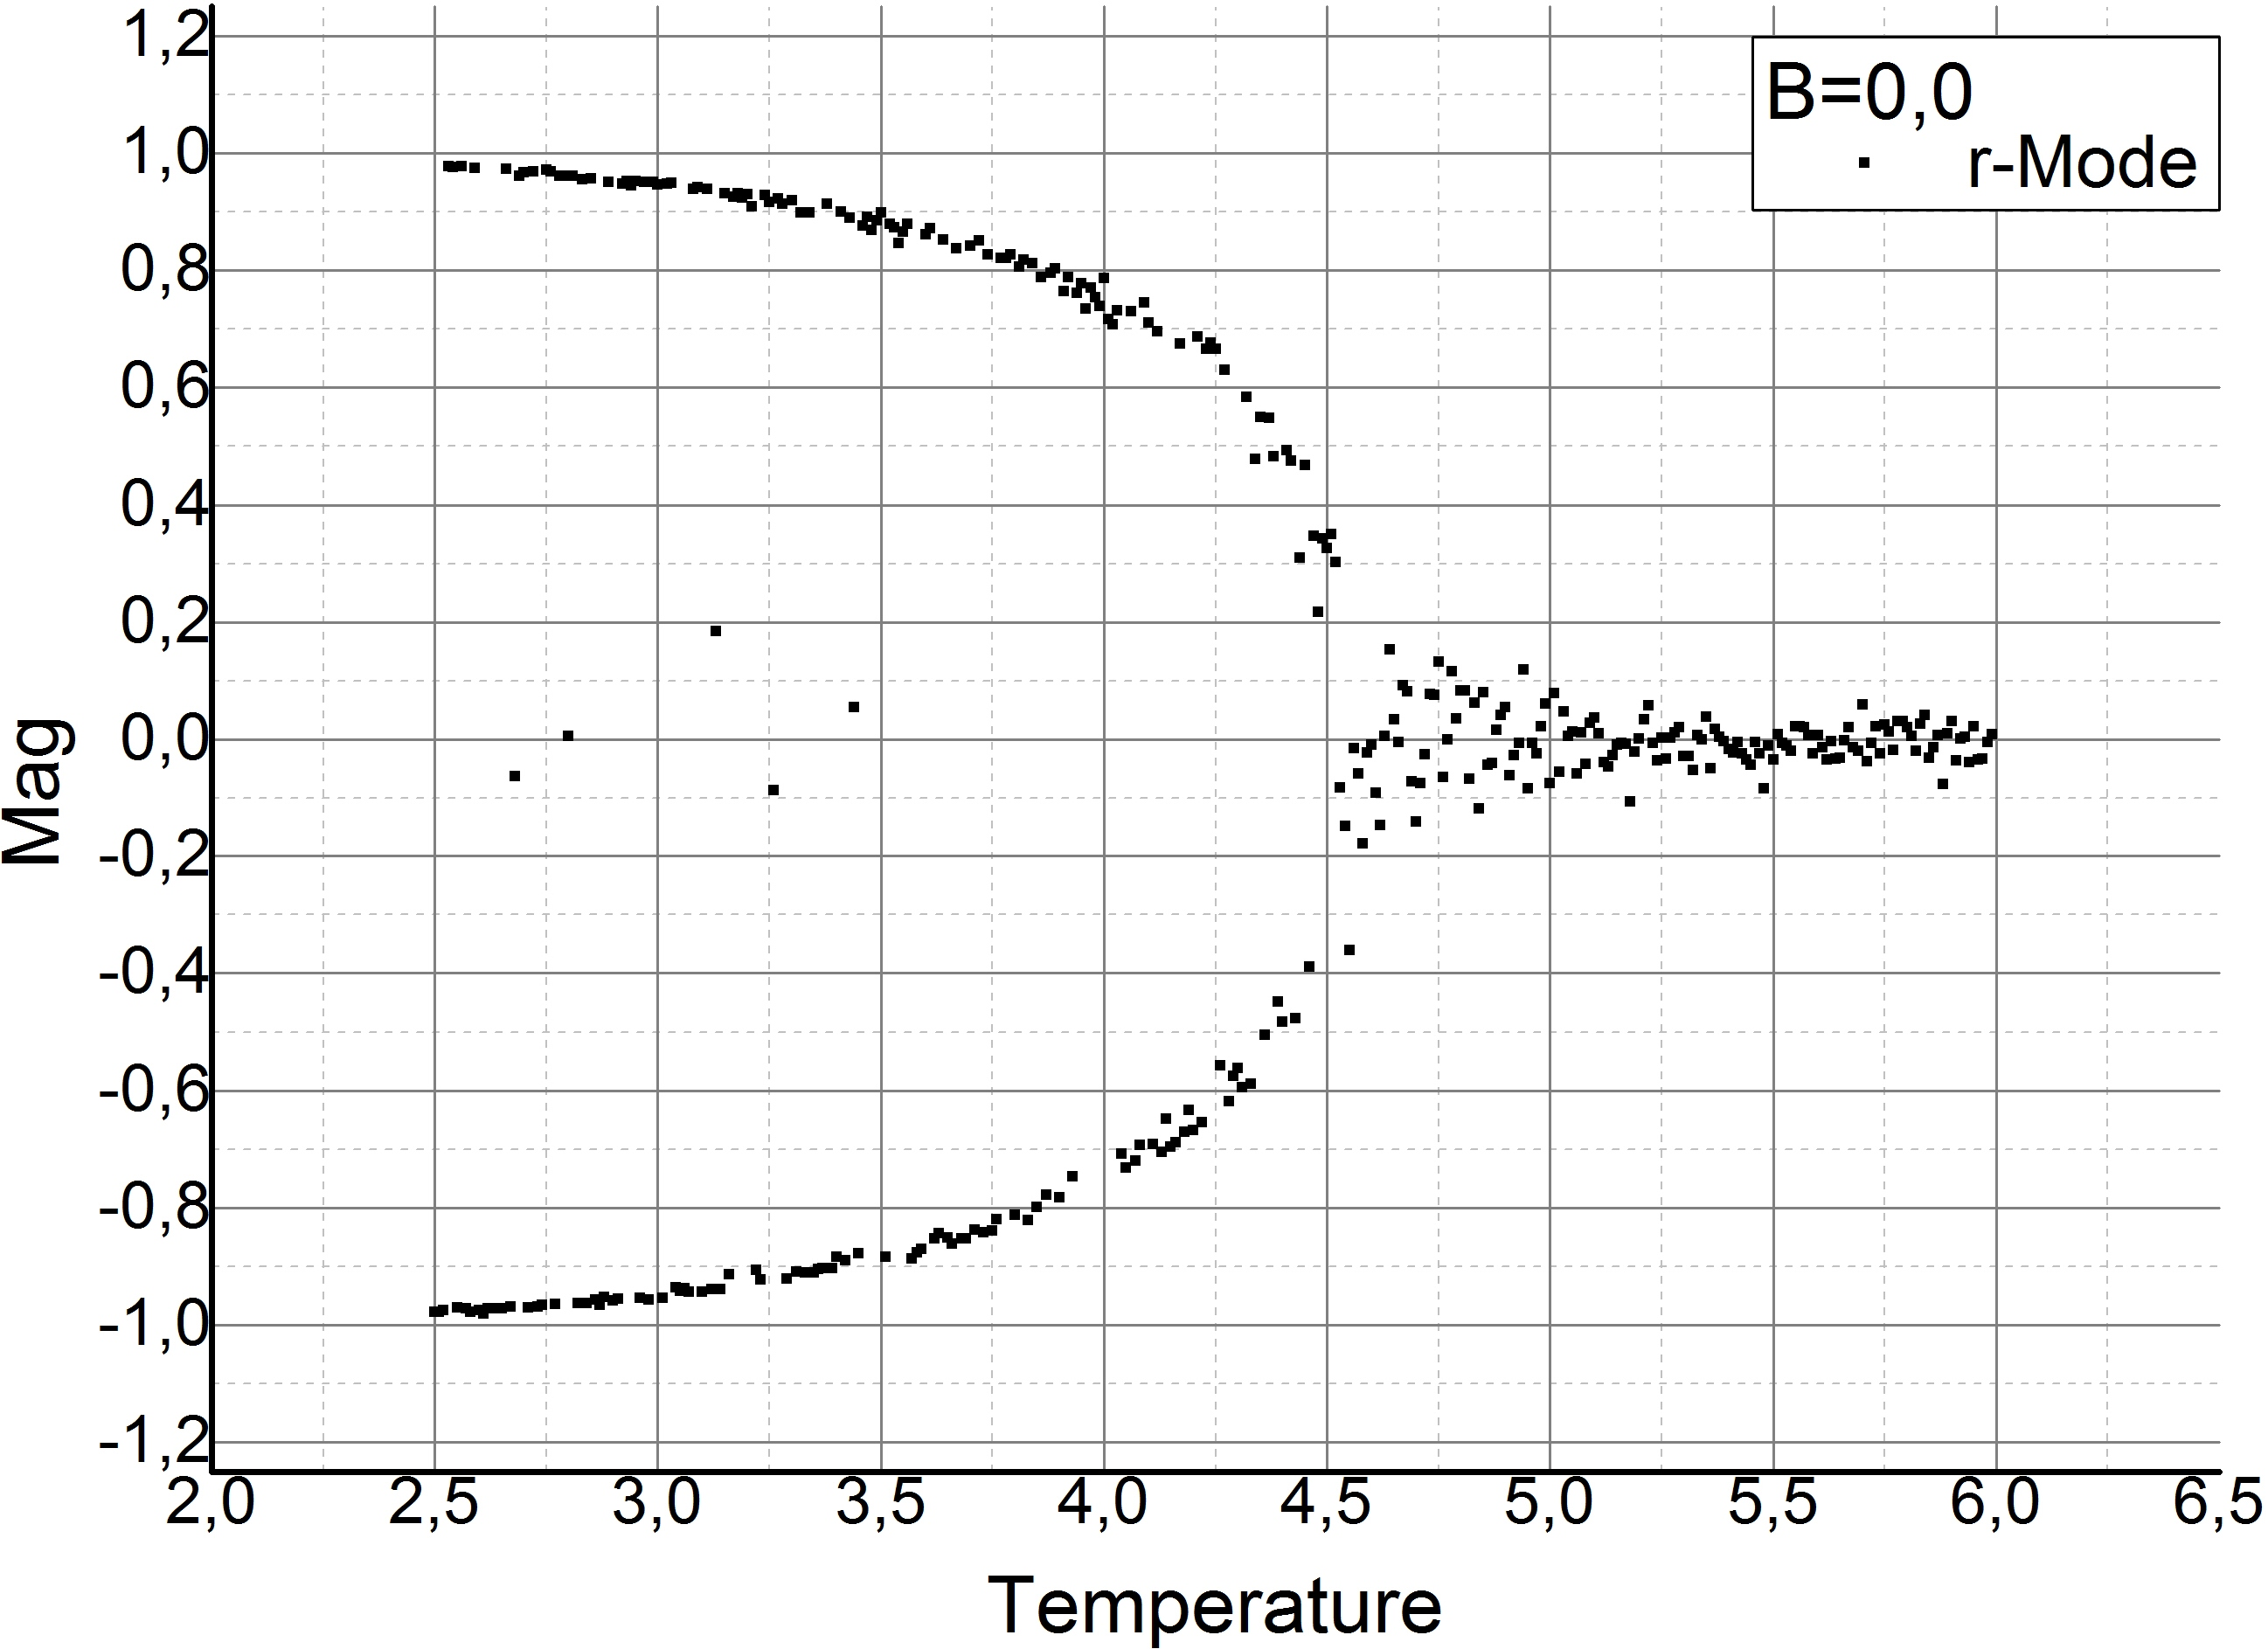
\includegraphics[width=0.47\textwidth]{../Graph_Export/MP3D/m(T)_B=0_rMode_MP3D_Plot.jpg}
}	
	\subfigure[Start aus geordneten Konfigurationen]{
		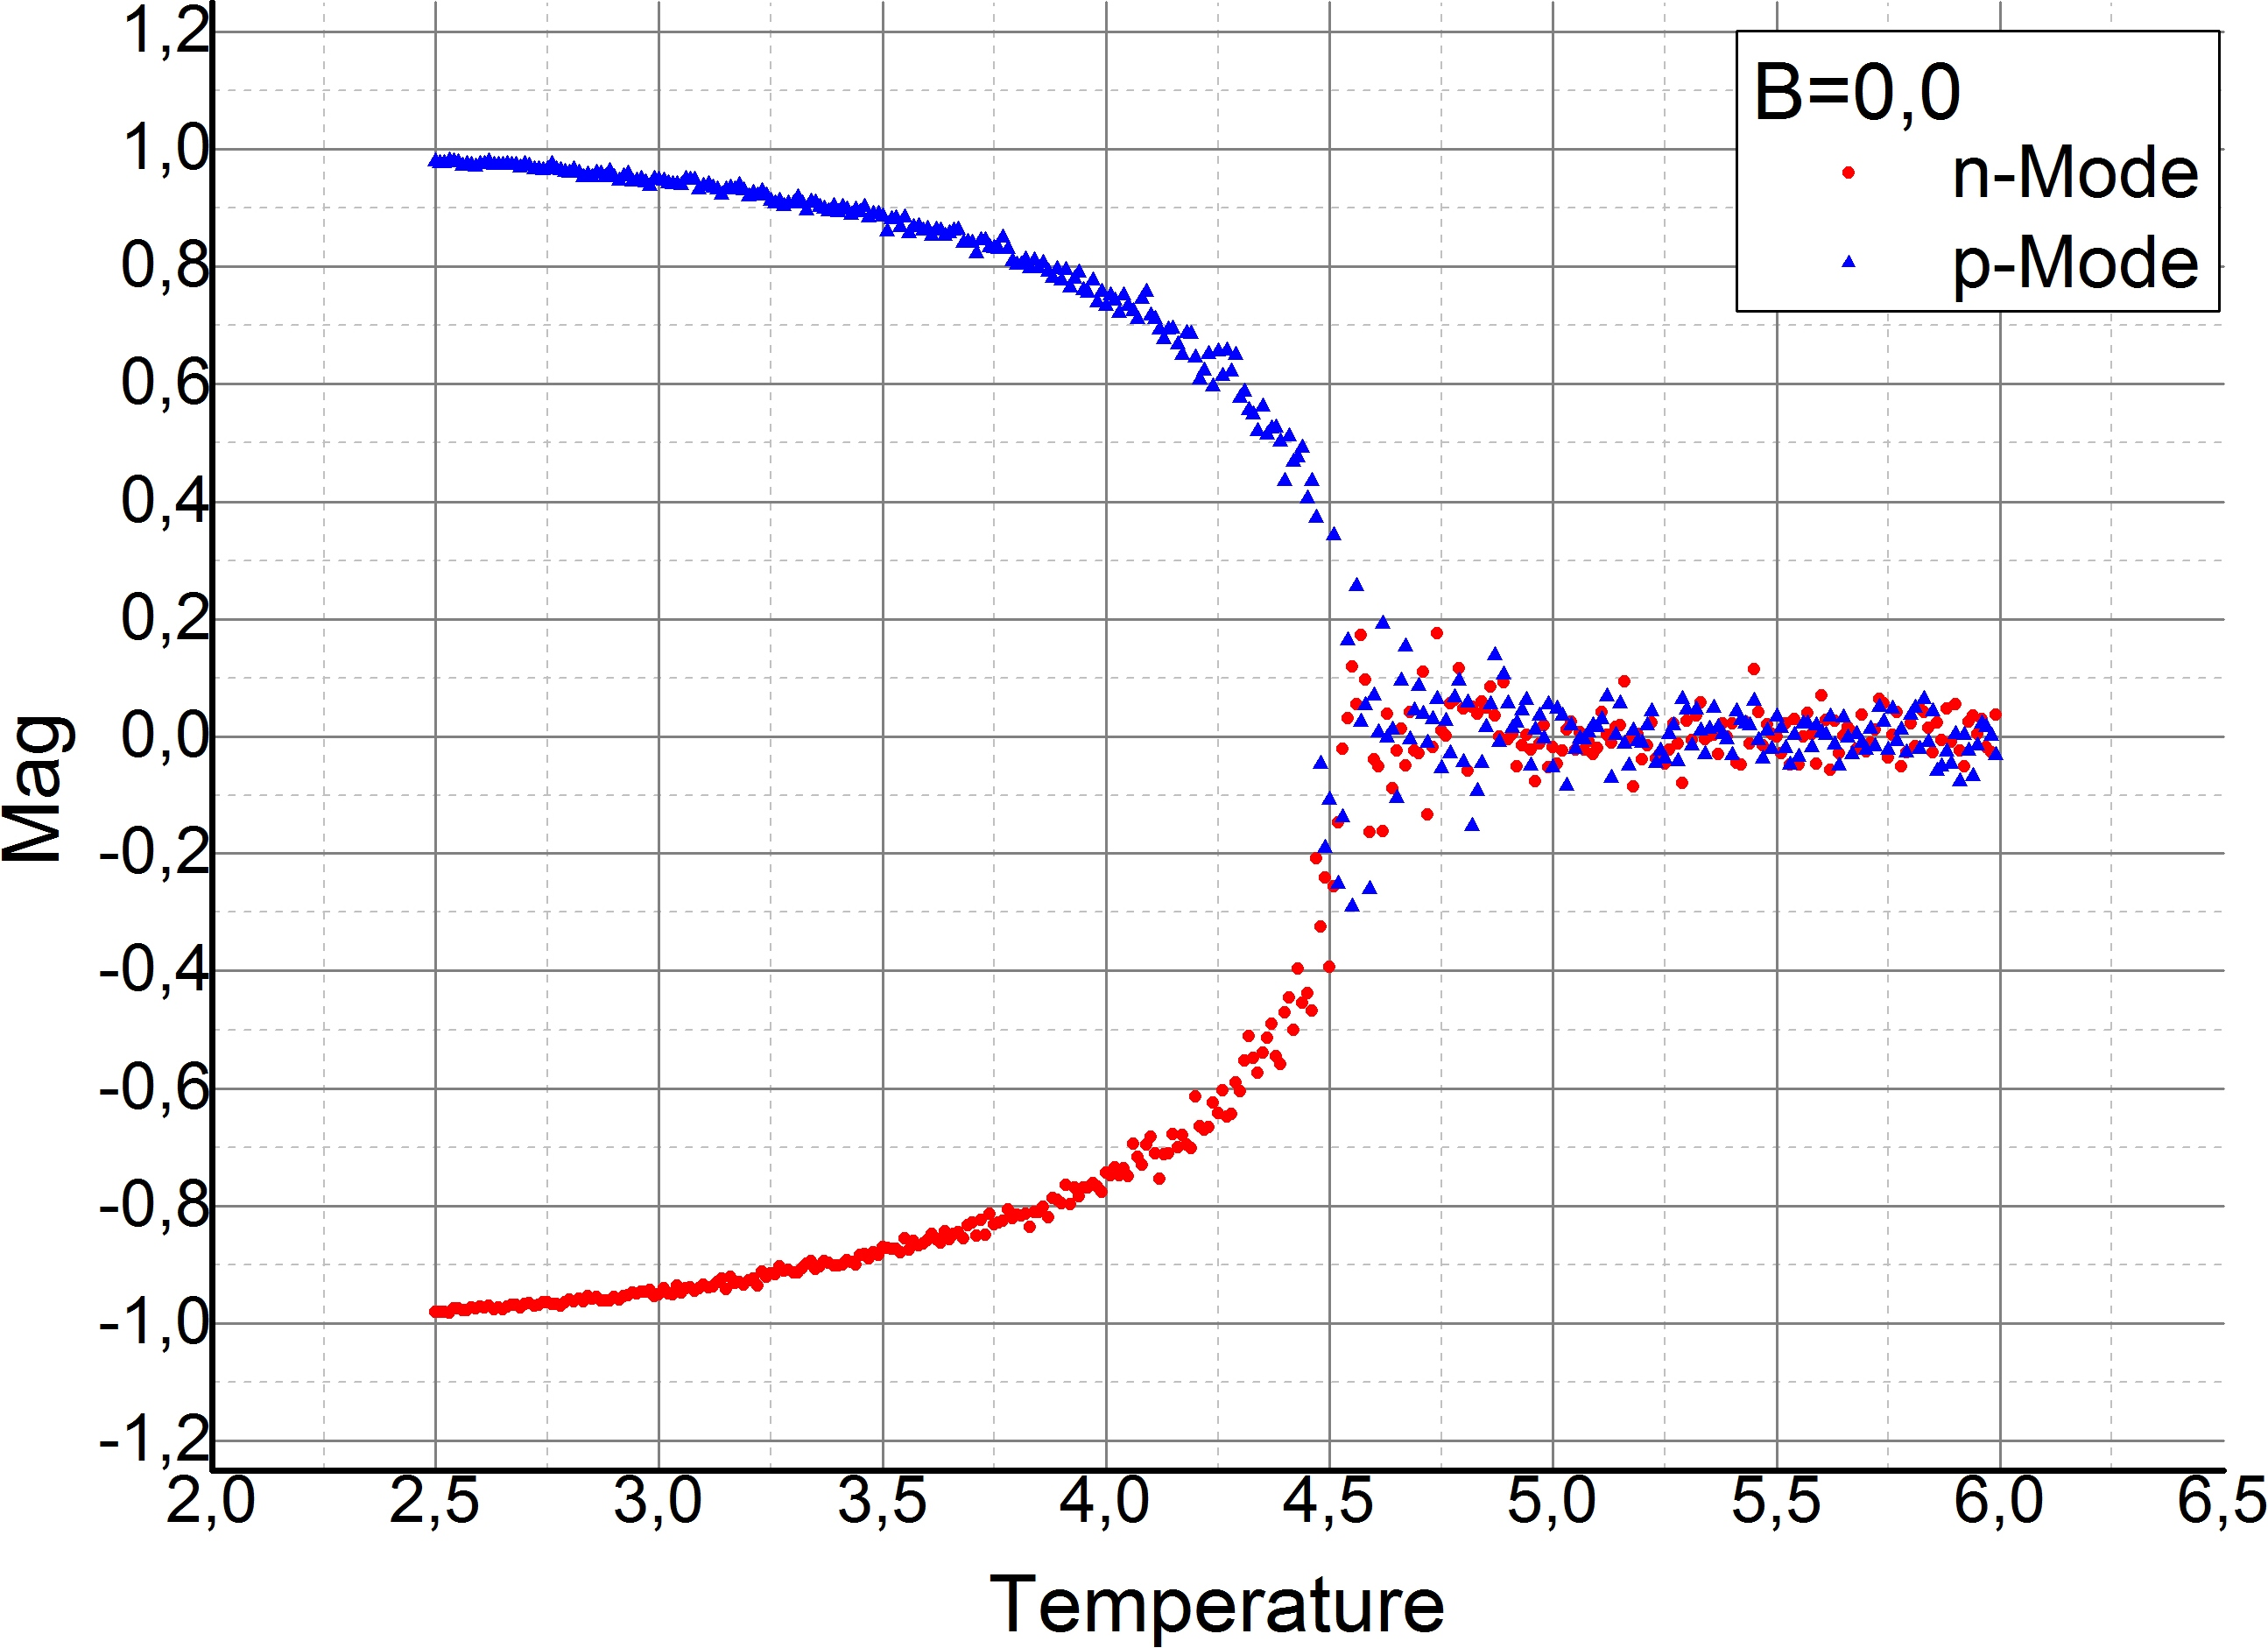
\includegraphics[width=0.47\textwidth]{../Graph_Export/MP3D/m(T)_B=0_pnModes_MP3D_Plot.jpg}
}		
	\caption{Temperaturabhängigkeit der Magnetisierung im 3D Ising Modells via Metropolisalgorithmus ohne äußeres Feld}
	\label{mp3d0modes}
\end{figure}
Es fällt auf, dass deutlich weniger Ausreißer im Bereich $T<T_{c}$ existieren und auch das Grundrauschen hat deutlich abgenommen. Es liegt nur noch bei etwa $\pm 0,1 = 0,2$. Ersteres liegt vermutlich an der kompakteren Struktur, also der höheren Anzahl an direkten Nachbarn. Zweiteres kommt durch die größere Anzahl an Spins (Gitterpunkten) zustande. Im 3D-Modell ist bei geeigneten Werten die Startkonfiguration auch für Simulationen ohne äußeres Feld zweitrangig. In beiden Fällen kann die Curie-Temperatur mit $T_{c}\approx 4,5\pm 0,02$ abgeschätzt werden.


Auch bei der Untersuchung der Einwirkung verschiedener äußerer Felder treten die gleichen Effekte analog zum 2D-Modell auf. Für die Simulation von $B=\pm 0,1$ wurden Temperaturen von $T=2,5$ bis $T=9,0$ mit Schrittweite $\Delta T= 0,02$ und für $B=\pm 0,4$ Temperaturen von $T=2,5$ bis $T=12,0$ mit Schrittweite $\Delta T= 0,025$ betrachtet.
 \begin{figure}[H]
	\centering
	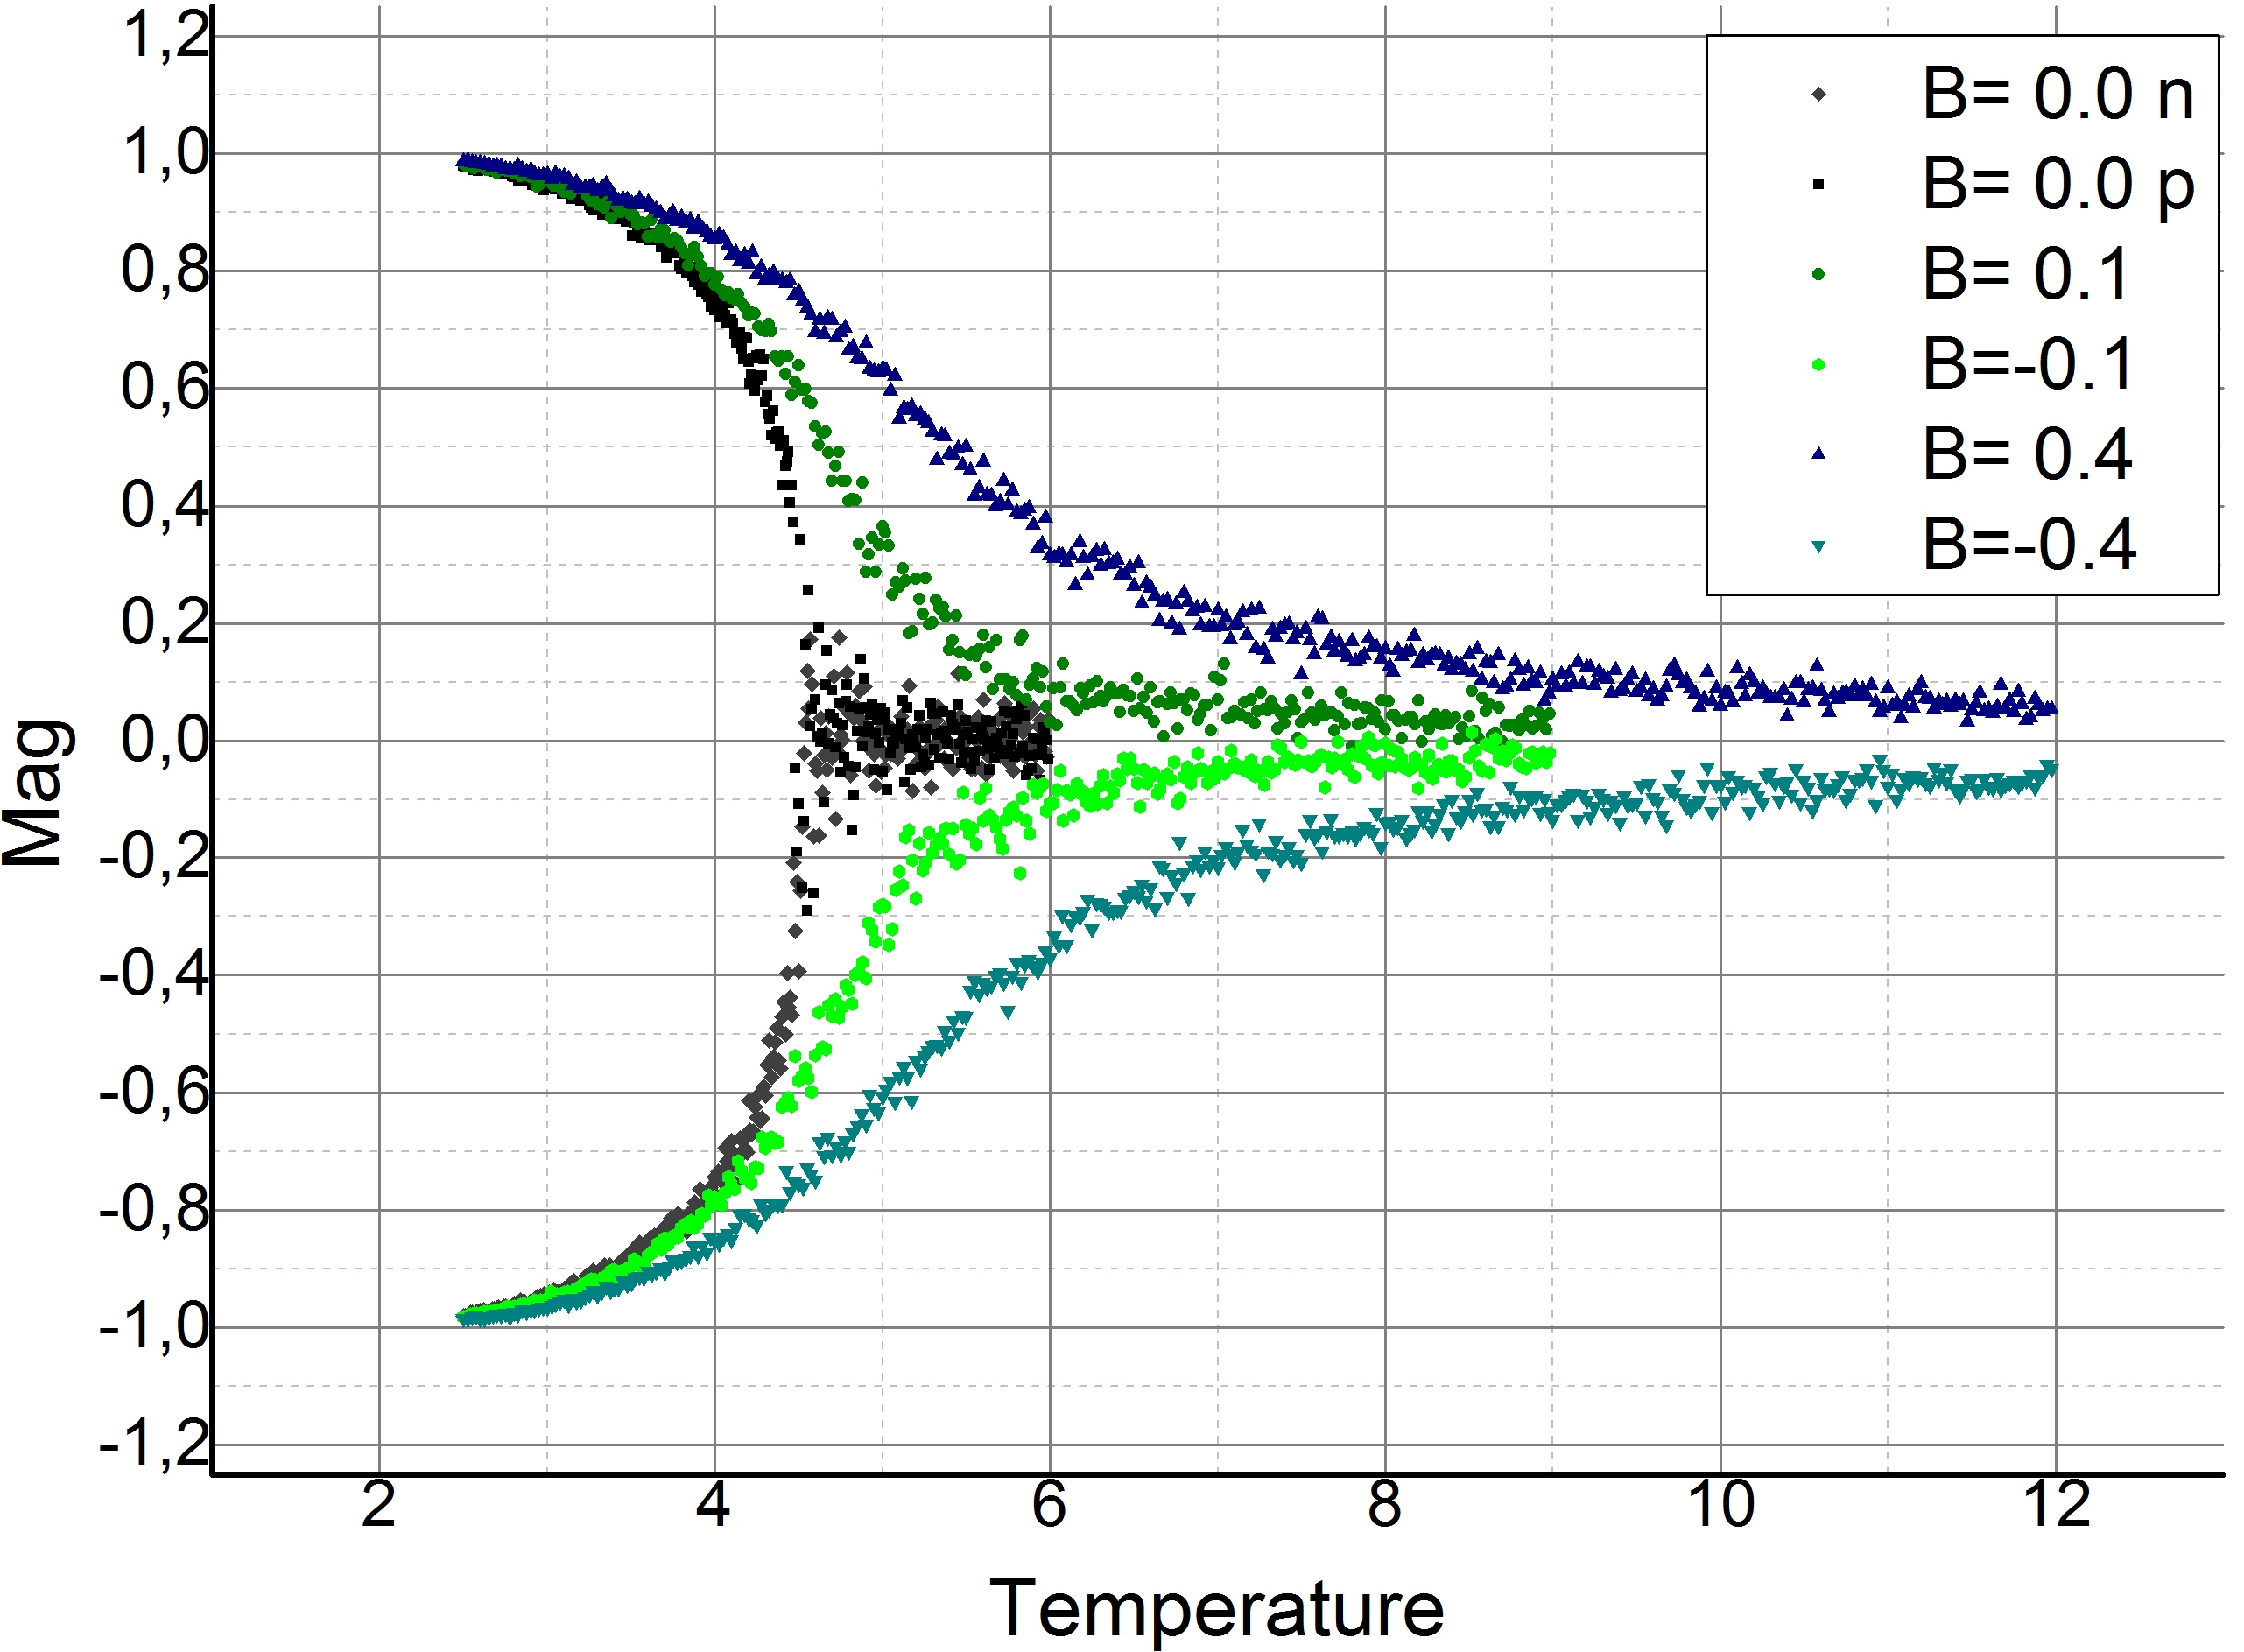
\includegraphics[width=0.8\textwidth]{../Graph_Export/MP3D/m(T)_MP3D_Plot.jpg}	
	\caption{Temperaturabhängigkeit der Magnetisierung im §D Ising Modells via Metropolisalgorithmus für verschiedene äußere Felder}
	\label{mp3db}
\end{figure}


\subsection{Schaltverhalten im Magnetfeld}

Bilder, Bilder, Bilder...
